%!TEX root=../document.tex

\section{Ergebnisse}

	\subsection{Installieren von Docker auf Arch Linux}
		\subsubsection{Vorbereitung}
			Die Installation von Docker auf Arch Linux kann auf zwei verschiedene Arten durchgeführt werden. Entweder über das Community-package oder über das package aus dem AUR. Docker benötigt verschiedene Dependencies:
			\begin{itemize}
				\item bridge-utils
				\item device-mapper
				\item iproute2
				\item sqlite
			\end{itemize}
			
		\subsubsection{Installation}
		Um das normale package zu installieren reicht ein simples
		\begin{lstlisting}[language=bash,caption={Installieren des Docker packages über Pacman}]
		$ sudo pacman -S docker
		\end{lstlisting}
		Oder im pack AUR
		\begin{lstlisting}[language=bash,caption={Docker aus dem AUR}]
		$ yaourt -S docker-git
		\end{lstlisting}
		
		\subsubsection{Starten von Docker}
		Nach der Installation wird ein \textbf{systemd} service erstellt und wird folgendermaßen gestartet:
		\begin{lstlisting}[language=bash,caption={Starten von Docker}]
		$ systemctl start docker
		\end{lstlisting}
		
	\subsection{Installieren eines Docker-Image}
		Um eine neues Docker-Projekt anzulegen  muss ein neuer Ordner angelegt werden und danach ein neues File erstellen mit dem Namen: \textbf{Dockerfile}
		\begin{lstlisting}[language=bash,caption={Erstellen des Docker-Project root}]
		$ mkdir dockerstuff
		$ cd dockerstuff
		$ nano Dockerfile
		\end{lstlisting}
		Zu Beginn fügt man nur den Namen des Images ein:
		\begin{lstlisting}[language=bash,caption={Dockerfile erster Eintrag}]
		$ FROM ubuntu
		\end{lstlisting}
		Jetzt kann das neue Image gebuilded werden. Dieser Befehl passiert mit einer Namensgebung
		\begin{lstlisting}[language=bash,caption={Builden des Images}]
		$ docker build -t testproj
		\end{lstlisting}
		Um eine Verbindung zum Docker-Container herzustellen muss er noch gestartet werden:
		\begin{lstlisting}[language=bash,caption={Starten des Containers}]
		$ docker run -it ubuntu
		\end{lstlisting}
	
	\subsection{MySQL auf der Docker-Machine}
		Um die manuelle Erstellung abzuschließen wird auf der Maschine noch ein Tutorial durchgeführt, wie man MySQL installiert.
		\href{https://www.digitalocean.com/community/tutorials/how-to-install-mysql-on-ubuntu-14-04}{MySQL-Installationsanweisung}
		
		\begin{lstlisting}[language=bash,caption={MySQL beim Start ausführen}]
		$ systemctl enable mysql
		\end{lstlisting}
	\subsection{Probleme}
	Um auf dem Docker-Container Packages installieren zu können muss zunächst ein \textbf{update und upgrade} des Systems vorgenommen werden.

	\subsection{Erstellen eines eigenen Dockerfile (Image)}
		\subsubsection{Syntax des Dockerfiles}
			Um das Dockerfile richtig zu konfigurieren müssen gewisse Syntax-Regeln eingehalten werden.
			\begin{itemize}
				\item \textbf{\# COMMENT} mit \# wird ein Kommentar eingeleitet
				\item \textbf{INSTRUCTIONS} Dieser Befehl hebt hervor, welche 	Parameter und andere Vorbereitung getroffen werden müssen um ein Dockerfile lauffähig zu machen.
				\item \textbf{FROM} Ist immer die erste Zeile, da es das Image festlegt welches verwendet wird.
				\item \textbf{MAINTAINER} Legt den Autor des Dockerfiles fest.
				\item \textbf{ENV} Setzt die Umgebungsvariablen in der Form [key] [value]. Der value kann irgendein String sein, zum Beispiel auch IP-Adressen, URLs.
				\item Es gibt verschiedene Varianten ein Umgebungsvariablen zu setzen: \textbf{ADD, COPY, ENV, EXPOSE, LABEL, USER, WORKDIR, VOLUME, STOPSIGNAL und ONBUILD.}
				\item \textbf{RUN} Führt ein command aus. Zum Beispiel führt \textbf{RUN apt-get update \&\& apt-get install mysql}, führt ein update durch und installiert mysql.
				\item \textbf{EXPOSE} Definiert den Port auf dem die Virtuelle Maschine laufen soll.
				\item \textbf{CMD} Kann nur einmal in einem Dockerfile vorkommen. Die Syntax ist \textbf{CMD [''executable'',"param1","param2"]}
				\item \textbf{ENTRYPOINT} beschreibt welcher command beim Start ausgeführt werden soll.
			\end{itemize}
		\subsubsection{Fertiges Dockerfile}
		
			\begin{lstlisting}[language=bash,caption={Dockerfile des selbsterstellten Images}]
			# Pull base image.
			FROM ubuntu:14.04
			
			# Install.
			RUN \
			sed -i 's/# \(.*multiverse$\)/\1/g' /etc/apt/sources.list && \
			apt-get update && \
			apt-get -y upgrade && \
			apt-get install -y build-essential && \
			apt-get install -y software-properties-common && \
			apt-get install -y byobu curl git htop man unzip vim wget && \
			apt-get install -y mysql-server && \
			rm -rf /var/lib/apt/lists/*
			
			# Set environment variables.
			ENV HOME /root
			
			# Define working directory.
			WORKDIR /root
			
			#RUN service mysql restart && /tmp/setup.sh
			
			# Define default command.
			ENTRYPOINT service mysql restart && bash
			\end{lstlisting}
		
		\subsubsection{Probleme}
		Damit die Installationsprompt automatisch durchgeführt wird kann man beim Installieren von Packages ein \textbf{-y} als Option hinzugefügt werden. Dies bewirkt eine \textbf{noninteractive-Installation}
		
	\subsection{Verbundene Images (Wordpress)}
		\subsubsection{Verwenden des Images}
		Ein lauffähiges \textbf{docker-compose} wird benötigt damit der Wordpress-Container funktioniert.
		
		\begin{lstlisting}[language=bash,caption={docker-compose.yml}]
		version: '2'
		
		services:
		
		wordpress:
		image: wordpress
		ports:
		- 8000:80
		environment:
		WORDPRESS_DB_PASSWORD: example
		
		mysql:
		image: mariadb
		environment:
		MYSQL_ROOT_PASSWORD: example
		\end{lstlisting}
					
		\begin{figure}[!h]
			\begin{center}
				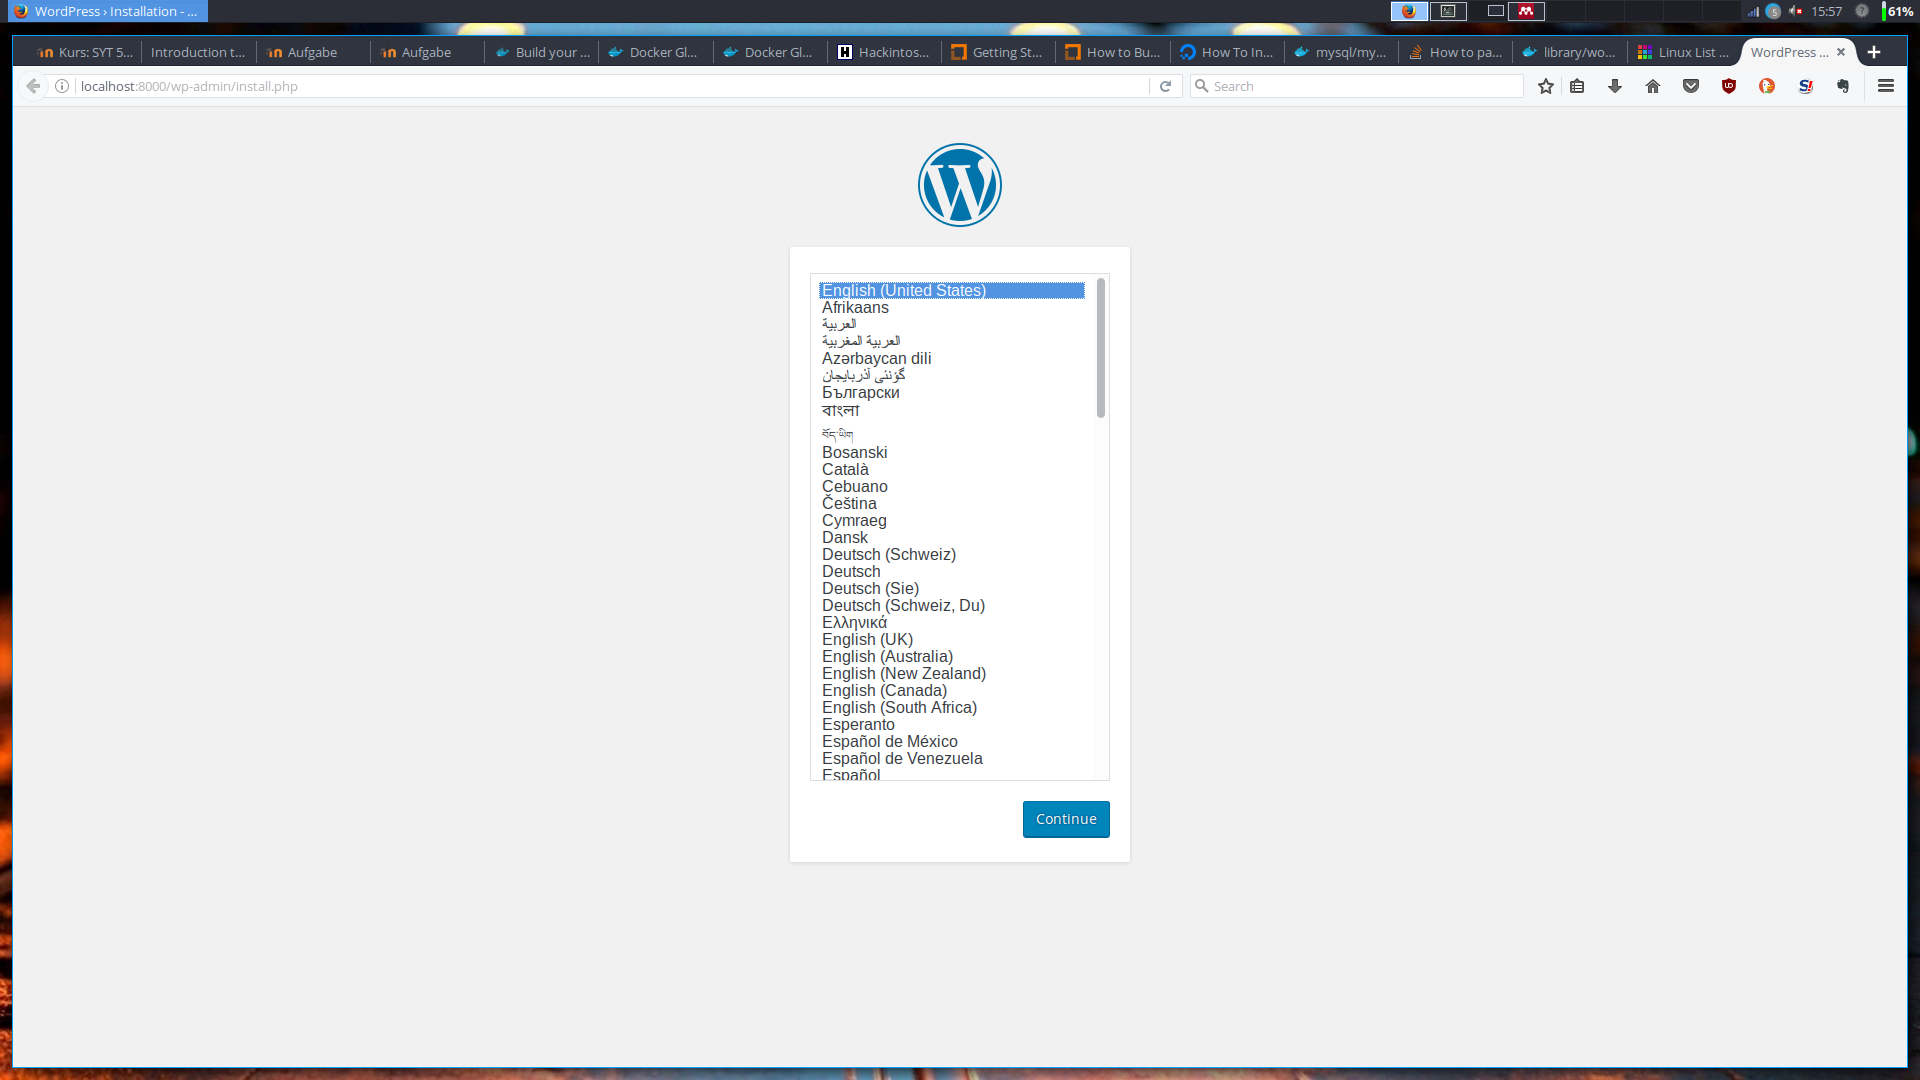
\includegraphics[width=0.8\linewidth]{images/wp}
				\caption{Ergebnis des Wordpress-Containers}
				\label{broker}
			\end{center}
		\end{figure}
		
		\subsubsection{Probleme}
		Damit der \textbf{docker-compose} einwandfrei funktioniert wird noch eine Dependency benötigt, da sonst diese Fehlermeldung auftritt:
				\begin{lstlisting}[language=bash,caption={pip Installationsanweisung}]
				$	pkg_resources.DistributionNotFound: The 'colorama>=0.3.7' distribution was not found and is required by docker-compose
				\end{lstlisting}

		Die Fehlermeldung wird behoben, indem man ein Package mit dem \textbf{Python Installer pip} installiert.
		\begin{lstlisting}[language=bash,caption={pip Installationsanweisung}]
		$	pip install colorama
		\end{lstlisting}
		
\section{Quellen}

Wordpress-Docker: \url{ https://hub.docker.com/_/wordpress/}

Docker-Setup:\url{https://www.linux.com/news/getting-started-docker}

Docker-Image:\url{ https://www.linux.com/learn/how-build-your-own-custom-docker-images}

Docker-Arch Linux: \url{http://docs-stage.docker.com/engine/installation/linux/archlinux/}
		
	
		
		
		
	